%%%%%%%%%%%%%%%%%%%%%%%%%%%%%%%%%%%%%%%%%%%%%%%%%%%%%%%%%%
%%
%%  LOD-L10.tex
%%  Lecture 10: Symplectic Mechanics and Diffeology
%%
%%%%%%%%%%%%%%%%%%%%%%%%%%%%%%%%%%%%%%%%%%%%%%%%%%%%%%%%%%

\chapter*{\S L10. Symplectic Mechanics and Diffeology}
\setcounter{footnote}{0}

%%%%%%%%%%%%%%%%%%%%%%%%%%%%%%%%%%%%%%%%%%%%%%%%%%%%%%%%%%
%%
%% MARK: Abstract
%%
%%%%%%%%%%%%%%%%%%%%%%%%%%%%%%%%%%%%%%%%%%%%%%%%%%%%%%%%%%
\begin{abstract}
  I give,
  in this lecture,
  a short survey on symplectic mechanics.
  The basic foundations in the work of Lagrange at the end of the 18th century and the beginning of the 19th,
  and what it became in the middle of the 20th century with what it is called now:
  \emph{symplectic mechanics}.
  We will discuss also how to extend these constructions to Diffeology,
  the main concepts.
\end{abstract}

%%%%%%%%%%%%%%%%%%%%%%%%%%%%%%%%%%%%%%%%%%%%%%%%%%%%%%%%%%
%%
%% MARK: Introduction
%%
%%%%%%%%%%%%%%%%%%%%%%%%%%%%%%%%%%%%%%%%%%%%%%%%%%%%%%%%%%

There are a few different approaches to symplectic geometry in mechanics.
At the beginning there are three papers from Joseph-Louis Lagrange in 1808, 1809 and 1810 \cite{Lag08,Lag09,Lag10}:

1) {\em Sur la th\'eorie des variations des \'el\'ements des plan\`etes et en particulier des variations des grands axes de leurs orbites} (1808).

2) {\em Sur la th\'eorie g\'en\'erale de la variation des constantes arbitraires dans tous les probl\`emes de la m\'ecanique}(1809).

3) {\em Second m\'emoire sur la th\'eorie g\'en\'erale de la variation des constantes arbitraires dans tous les probl\`emes de la m\'ecanique} (1810).

In these papers,
Lagrange sets the first elements of what we can call ``symplectic calculus''.
The question was the stability of the great axes of the planets,
and Lagrange brought a simplification in the approximation computations of this time,
in particular by Laplace and Poisson.
I will not write down here the details of his work but I refer (for now) to the paper I wrote on the subject:
{\em Les Origines du Calcul Symplectique chez Lagrange},
but in French \cite{PIZ98}.

That said,
I will emphasize
---~in this overview on symplectic mechanics~---
the following points relative to the global structure of the spaces of solutions of dynamical (symplectic) systems.

\begin{enumerate}
  \item The presymplectic/symplectic framework.
  \item The symmetries of dynamical systems.
  \item Isolated mechanical/dynamical systems, the Galilean and Poincaré groups.
  \item The moment map associated to a group of symmetries.
  \item The conservation of the moment map (Noether-Souriau theorem).
  \item The Souriau cocycle and the barycentric decomposition.
  \item The elementary particles/systems and the classic spin.
  \item The ``geometric quantization program'', the prequantization.
\end{enumerate}

These few points summarize,
I believe,
the main progress on the global structure of dynamical systems made in the 20th century.

Of course,
symplectic mechanics does not reduce to these chapters,
other constructions like the behavior of hamiltonian vector fields,
the geometric optics,
reflexion,
diffraction,
caustics\dots
The structure of the group of symplectomorphisms,
etc.
All these subjects are a part of modern symplectic mechanics.
A whole year of lectures could hardly be enough to cover all the applications of symplectic mechanics.


%%%%%%%%%%%%%%%%%%%%%%%%%%%%%%%%%%%%%%%%%%%%%%%%%%%%%%%%%%
%%
%% MARK:  The short Approach To Symplectic Mechanics
%%
%%%%%%%%%%%%%%%%%%%%%%%%%%%%%%%%%%%%%%%%%%%%%%%%%%%%%%%%%%
\section{The short approach to symplectic mechanics}

The following presentation of the symplectic structure on the space of solutions of a dynamical (second order differential equation) system is due to Elie Cartan \cite{Car22},
followed by some authors,
Galissot \cite{Gal52},
and especially Jean-Marie Souriau in his book ``Structure des Systèmes Dynamique'' \cite{Sou70}.

\begin{Article}{To drive out the denominators.}{}
  Let us recall that a classical dynamical system in Galilean Mechanics,
  or Newtonian Mechanics,
  is described by an ordinary second order differential equation.
  For example,
  for a material point:
  $$%
    m{d^2x \over dt^2}
    = F(x,v,t)
    \SpacedText{where} v = {dx \over dt}.
    $$%
  The unknown here is the path $[t \mapsto x]$,
  where $t$ is a real number defined on some interval and $x \in \RR^3$.
  
  Then we transform this second order system into a first order differential equation system:
  $$%
    m{dv \over dt}
    = F(x,v,t)
    \SpacedText{and}
    v = {dx \over dt}.
    $$%
  Then we reinterpret the Newton equations by ``driving out the denominators'':
  $$%
    m dv = F(x,v,t) dt
    \SpacedText{and}
    dx = v dt.
    $$%
  We need here to explain this writing.
  Consider the subset
  $$%
    Y \subset \RR^3 \times \RR^3 \times \RR
    $$%
  where $F$ is defined.
  We call it the space of initial conditions,
  or following Souriau:
  the ``evolution space''.
  Let $y= (x,v,t)$ a point in $Y$,
  let us denote by $dy$ a tangent vector to $Y$, at the point $y$,
  that is a vector of $\RR^7$.
  We can imagine $dy$ being the shortcut the derivative of a path $s \mapsto y$
  $$%
    dy = {dy \over ds} \in T_yY
    \SpacedText{with}
    dy = \Vector{dx \\ dv \\ dt}.
    $$%
  Then,
  the equations of motion writes
  $$%
    m dv - F(x,v,t) dt =0
    \SpacedText{and}
    dx -vdt =0.
    $$%
  At this point we use a trick,
  and considering another tangent vector
  $$%
    \delta y = \Vector{\delta x \\ \delta v \\ \delta t} \in T_yY,
    $$%
  we define
  $$%
    \omega(dy,\delta y) = \langle m dv - F dt, \delta x - v \delta t\rangle
    - \langle m \delta v - F \delta t,  dx - v dt\rangle.
    $$%
  Let us make some comment on the notation:
  first of all,
  $F$ denotes at the same time the function $F$ and the value of $F$ at the point $y=(x,v,t)$.
  Second of all,
  the $2$-form $\omega$ should rigorously be indexed by the point $y$ where it is taken,
  but the vectors $dy$ and $\delta y$ already contain this information,
  so it is unnecessary to be redundant.
  
  One can check now that:
  
  \begin{enumerate}
    \item $\omega$ is a $2$-form on $Y$.
    \item the vector $dy \simeq dy/ds$ satisfies the \emph{equations of motion} if and only if it belongs to the kernel of $\omega$.
  \end{enumerate}
  
  The kernel of $\omega$ is defined by
  $$%
    dy \in \ker(\omega) \quad \Leftrightarrow \quad \omega(dy,\delta y) = 0 \quad \forall \delta y.
    $$%
  
  Therefore,
  the \smuline{integral curves} of the kernel distribution
  $$%
    y \mapsto \ker(\omega)
    $$%
  are the solutions of the Newton equations.
  
  \uline{Proposition 1.}~{\itshape The space $\cM$ of integral curves of the kernel distribution is a manifold,
  that can be,
  for some kind of force $F$,
  non Hausdorff.
  It is called the \emph{space of motions}.}
  
  I would like to emphasize the fact that a solution of the differential equation,
  in this approach, is an integral curve of the distribution $y \mapsto \ker(\omega)$,
  that is,
  a subset of $Y$,
  the graph of some curve $t \mapsto (x,v,t)$.
  So the space of motions is indeed a set of subspaces of $Y$,
  and this set of subspaces is equipped with a structure of manifold.
  
  \uline{And beware} to not confuse the motion with the trajectory of the motion.
  The schedule of the trajectory is a part of the motion.
  For example,
  a circular motion has a circle for trajectory but its motion is a line,
  precisely a helix.
  That is why it is not enough to know the route of the bus to take advantage of it,
  you have to know when it stops in front of your door.
  The timetable is an element of the movement.
  
  \uline{Proposition 2.} {\itshape The restrictions $(x,v) \mapsto \Class_t(x,v)$,
  for all $t \in \RR$,
  make a canonical atlas of the manifold $\cM$.}
  
  Note that these canonical charts $\Class_t$ are called \emph{Darboux charts} because the symplectic form takes the canonical expression,
  $$%
    \omega_t = m \sum_{i=1}^3 dx_i \wedge dv_i.
    $$%
  
  \uline{Proposition 3.} {\itshape If the force $F$ is the gradient of some \emph{potential} $\pphi$,
  actually $F = - \grad(\pphi)$,
  then the $2$-form $\omega$ is closed
  $$%
    d\omega = 0,
    $$%
  and descends on the quotient space $\cM$ into a symplectic $2$-form.}
  
  In that case,
  the $2$-form $\omega$ is the exterior derivative of the so-called \emph{Cartan form}
  $$%
    \lambda(\delta y) = m \langle v,\delta x\rangle - h\, \delta t
    \SpacedText{with}
    h = {1 \over 2} m \Norm{v}^2 + \pphi.
    $$%
  \uline{Definition.}{\itshape We recall that a symplectic form on a manifold is a \uline{non degenerate closed $2$-form}.}
\end{Article}

%%%%%%%%%%%%%%%%%%%%%%%%%%%%%%%%%%%%%%%%%%%%%%%%%%%%%%%%%%
%%
%% MARK:  Presymplectic and Symplectic Manifolds
%%
%%%%%%%%%%%%%%%%%%%%%%%%%%%%%%%%%%%%%%%%%%%%%%%%%%%%%%%%%%
\section{Presymplectic and symplectic manifolds}

\begin{Article}{Presymplectic form.}{}
  Let $M$ be a manifold,
  a closed $2$-form $\omega$ on $M$ is said to be \emph{presymplectic} if its kernel has a constant dimension on $M$ \cite{Sou70}.
  The vector distribution
  $$%
    y \mapsto \ker(\omega)
    $$%
  is called the \emph{characteristic distribution}.
  Thanks to the Frobenius theorem that states that for every differential form $\omega$,
  the characteristic distribution
  $$%
    y \mapsto \ker(d\omega) \cap \ker(\omega)
    $$%
  is integrable,
  since $\ker(d\omega)_y = T_yM$,
  the characteristic distribution of a  closed form $y \mapsto \ker(\omega)$ is integrable.
  
  The leaves of the integral submanifolds of the characteristic distribution are called \emph{characteristics} of the distribution,
  and the resulting foliation is called the \emph{characteristic foliation}.
  
  The characteristics of the presymplectic form $\omega$ are the connected submanifolds $F \subset M$ such that at each point $y \in F$,
  $$%
    T_yF = \ker(\omega).
    $$%
\end{Article}

\begin{Article}{Symplectic dynamical systems.}{}
  In \emph{symplectic mechanics},
  a dynamical system is defined as a presymplectic manifold $(M,\omega)$.
  By analogy with the case of a particle,
  we call \emph{motions} of the system the characteristics of the presymplectic form.
  The \emph{space of motions},
  which plays an important role in mechanics,
  is then the set of all characteristics.
  
  \uline{Note.} There is no reason that,
  in general,
  the space of motions inherits a manifold structure by quotient,
  and it does not.
  That can be an obstacle in ordinary differential geometry,
  but not from the general diffeology point of view,
  where any case can be dealt with.
  The space of characteristic of a presymplectic manifold can always be equipped with the quotient diffeology,
  for which the usual diffeological tools continue to work.
  We denote this space by
  $$%
    \cM = M/ \ker(\omega).
    $$%
\end{Article}

\begin{Article}{Symplectic form.}{}
  A closed $2$-form $\omega$ on a manifold $M$ is said to be symplectic if it is \emph{non degenerate},
  that is,
  if its kernel is reduced to $\{0\}$
  $$%
    \omega \text{ symplectic }
    \quad \Leftrightarrow \quad
    d\omega = 0  \text{ and } \ker(\omega) = 0.
    $$%
  A symplectic manifold is then a presymplectic manifold with a trivial characteristic foliation:
  $$%
    F_y = \{y\}.
    $$%
  \smuline{Proposition.} Consider a presymplectic manifold $(M,\omega)$,
  if the quotient space $\cM = M / \ker(\omega)$ is a manifold,
  it inherits a symplectic form for which $\omega$ is the pullback.
  
  That is why symplectic geometry is important in physics:
  
  \begin{enumerate}
    \item Conservative dynamical systems are identified as presymplectic dynamical systems,
    for which the characteristic leaves are the solutions,
    or motions,
    of the system.
    \item The space of solutions of a conservative dynamical system,
    if it is a manifold itself,
    inherits a symplectic structure.
  \end{enumerate}
  
  The word ``conservative'' will be explained later.
\end{Article}

\begin{Article}{Example: The geodesics trajectories on the Sphere.}{}
  Consider the sphere $\Sph^2$.
  Let $\UnitBundle{\Sph^2}$ be the unitary tangent bundle:
  $$%
    \UnitBundle{\Sph^2} = \{ (x,u) \in \RR^3 \times \RR^3 \mid \Norm{x} = \Norm{u} = 1 \text{ and } \langle x, u \rangle =0 \}.
    $$%
  Define on $\UnitBundle{\Sph^2}$ the $1$-form
  $$%
    \lambda_y(\delta y) = \langle u, \delta x \rangle,
    \SpacedText{with}
    \left\{
    \begin{array}{rcl}
    y & = & (x,u) \in \UnitBundle{\Sph^2} \\
    \delta y & = & (\delta x, \delta u) \in T_y\UnitBundle{\Sph^2}.
    \end{array}
    \right.
    $$%
  let $\omega = d\lambda$,
  precisely
  $$%
    \omega_y(\delta y,\delta'y) = \langle \delta u, \delta' x \rangle - \langle \delta' u, \delta x \rangle.
    $$%
  One can check that $\omega$ is presymplectic and its characteristic distribution is defined by
  $$%
    {dy \over ds} \in \ker \omega
    \quad \Leftrightarrow \quad
    {dx \over ds} = \alpha u
    \SpacedText{and}
    {du \over ds} = - \alpha x,
    $$%
  for all $\alpha \in \RR$.
  The solutions of this system are great circles described by the \emph{law of motion}
  $$%
    x(s) = e^{sj(\ell)}x_0
    \SpacedText{and}
    u(s) = e^{sj(\ell)}u_0
    \SpacedText{with}
    \ell = x_0 \wedge u_0.
    $$%
  Note that $\ell = x \wedge u$ is constant on the solutions,
  it is called the \emph{kinetic momentum}.
  It is a particular case of the general moment map theory we will talk about later in the following.
  
  Thus,
  the map
  $$%
    y = (x,u) \mapsto \ell = x \wedge u
    $$%
  from $Y$ to $\Sph^2$ realizes the quotient space
  $$%
    Y / \ker(\omega) \simeq \Sph^2.
    $$%
  And the symplectic structure of the space of motions is equal,
  up to some constant,
  to the standard \emph{area form}
  $$%
    \Surf_\ell(\delta \ell, \delta' \ell) = \langle \ell,\delta \ell \wedge \delta' \ell \rangle.
    $$%
  This example is a special case of the general construction of the set of \emph{geodesic trajectories},
  which are equipped with a symplectic structure as soon as it is a manifold.
\end{Article}

\begin{Article}{Example: The geodesics trajectories on the torus.}{}
  The geodesic trajectories of the $2$-torus $\Torus^2 = \RR^2/\ZZ^2$ are the projections of the affine lines in $\RR^2$.
  Consider the projection which associates with each geodesic trajectory $\Delta$,
  its direction $u \in \Sph^1$.%
  \footnote{We consider first the oriented geodesic trajectories.}
  This is a surjection.
  We can write it
  $$%
    \pi \colon \fG_{\traj} \to \Sph^1
    \SpacedText{with} \pi(\Delta) = u.
    $$%
  Now,
  the fiber over the direction $u \in \Sph^1$ are all the projections on the $2$-torus $\Torus^2$ of the affine lines in $\RR^2$,
  parallel to the unique line of direction $u$,
  and passing through the origin.
  Depending on the orientation,
  these lines cut the axis $oy$ or the axis $ox$ according to the action of $\ZZ \oplus \ZZ$
  $$%
    (n,m) \colon y \mapsto y + n + \tau m,
    $$%
  with
  $$%
    u = (\alpha,\beta),
    \text{ with } \alpha^2 + \beta^2 = 1,
    \text{ and } \tau = {\beta \over \alpha}.
    $$%
  Thus,
  $$%
    \pi^{-1}(u) \simeq \Torus_\tau,
    $$%
  where $\Torus_\tau$ is the torus of slope $\tau$.
  If $\tau$ is rational then $\Torus_\tau$ is diffeomorphic to the torus $\Sph^1$,
  otherwise it is not a manifold but a diffeological space called the \emph{irrational torus} (of slope $\tau$) \cite{DI83}.
  
  So,
  in the case of the torus the space of geodesic trajectories is not a manifold but at least a diffeological space.
  We prove further in the book that the canonical symplectic form on the space of geodesic curves (which is always a manifold) descends,
  in some sense,
  to the quotient $\fG_{\traj}$,
  as a differential closed $2$-form,
  according to the definition in diffeology.
  
  That example shows in particular the necessity to enlarge the category of manifolds if we want to describe a bigger class of dynamical systems than usually.
\end{Article}

\begin{Article}{Darboux theorem.}{}
  An important theorem due to the mathematician Jean Gaston Darboux makes explicit the local nature of presymplectic and symplectic manifolds.
  Let $(M, \omega)$ be a presymplectic manifold of rank $2n$;
  the rank is defined by
  $$%
    \Rank(\omega) = \dim(M) - \dim(\ker(\omega)).
    $$%
  The rank of a $2$-form is always even,
  let $\dim(M) = 2n + k$.
  Then:
  
  There exists an atlas $\cA$ of charts such that,
  in any chart $F \in \cA$,
  the form $\omega$ can be identified with the matrix,
  if $k>0$:
  $$%
    \Vector{0_n & -\Id_n & 0 \\ \Id_n & 0_n & 0 \\ 0 & 0 & 0_k},
    \SpacedText{or}
    \Vector{0_n & -\Id_n \\ \Id_n & 0_n}
    $$%
  in the symplectic case $k=0$.
  
  This is an important,
  even crucial,
  theorem with an enormous set of applications.
  In a few words:
  a symplectic structure is \emph{flat},
  always.
  
  *~There is no local invariants. \\[.5ex]
  *~All symplectic invariants are global.
  
\end{Article}

%%%%%%%%%%%%%%%%%%%%%%%%%%%%%%%%%%%%%%%%%%%%%%%%%%%%%%%%%%
%%
%% MARK:  Symmetries and moment map
%%
%%%%%%%%%%%%%%%%%%%%%%%%%%%%%%%%%%%%%%%%%%%%%%%%%%%%%%%%%%
\section{Symmetries and moment map}

The symmetries of a dynamical system,
and its consequences,
are certainly at the heart of symplectic mechanics.

\begin{Article}{Symmetries of a system.}{}
  Let $(M,\omega)$ be a dynamical system,
  that is,
  a presymplectic manifold.
  We call a \emph{symmetry} of the system any diffeomorphism $f \in \Diff(M)$ that preserves the presymplectic form $\omega$.
  So,
  we define the largest group of symmetries of the system
  $$%
    \Diff(X,\omega) = \{ f \in \Diff(X) \mid f^*(\omega) = \omega \}
    $$%
  When the form is symplectic,
  such a diffeomorphism is called a \emph{symplectomorphism}.
  
  \smuline{Proposition.} {\itshape Except for trivial cases,
  the group $\Diff(X,\omega)$ is infinite dimensional.}
  
  \uline{Theorem.}~ {\it On symplectic manifolds,
  $\Diff(X,\omega)$ is transitive on $M$.
  Actually $\Diff(X,\omega)$ is $n$-transitive if $\dim(X) = 2n$ \cite{Boo69}.}
\end{Article}

\begin{Article}{Galilean mechanics.}{}
  The history has produced three kind of Mechanics,
  each of them characterized by a group of transformations \cite{PIZ18}.
  The \emph{Aristotelean group},
  the \emph{Galilean group} and the \emph{Poincaré group}.
  The Aristotelean mechanics has not been much developed.%
  \footnote{I have some project on this question.}
  The Galilean group is a $10$-dimensional Lie group,
  made of matrices
  $$%
    m = \Vector{A & b & c \\ 0 & 1 & e \\ 0 & 0 & 1}
    \SpacedText{with} A \in \SO(3); b,c \in \RR^3 \text{ and } e \in \RR.
    $$%
  This group is associated with Galilean/Newtonian mechanics.
  It acts on $\RR^3 \times \RR$ by
  $$%
    \Vector{A & b & c \\ 0 & 1 & e \\ 0 & 0 & 1}\Vector{r \\ t \\ 1} = \Vector{Ar + bt + c \\ t +e \\ 1}
    $$%
  Now we can answer the Question:
  
  \emph{What is a (Galilean) isolated system?}
  
  \uline{Principle} {\itshape An isolated Galilean system is a presymplectic manifold $(M,\omega)$ with a symmetric action of the Galilean group.}
  
  Later we will see that one adds the condition for this action to be Hamiltonian.
\end{Article}

\begin{Article}{Relativity and the Poincaré Group.}{}
  The group of Einstein Relativity is the Poincaré Group,
  that is,
  the group of affine transformations that preserve the quadratic form
  $$%
    ds^2 = c^2 dt^2 - dx^2 - dy^2 -dz^2,
    $$%
  with $(x,y,z,t) \in \RR^3 \times \RR$.
  $$%
    g : X \mapsto  LX + C,
    $$%
  where $X \in \RR^3 \times \RR$,
  $C \in \RR^4$ and $L$ is a linear automorphism of $ds^2$,
  a \emph{Lorentz transformation}.
  Let $X = (r,t) \in \RR^3 \times \RR$,
  every element of the Lorentz group decomposes uniquely in the product of 2 matrices
  $$%
    L= \Vector{\Id_3 & \bbeta \\ \bar \bbeta & 1}
    \Vector{B^{-1} & 0 \\ 0 & a},
    \text{ with } \bar B B + \bbeta \, \bar \bbeta = \Id_3
    \text{ and } \ a = \pm {1 \over \sqrt{1-\beta^2}}.
    $$%
  $B$ is a $3\times 3$ matrix,
  $\bbeta$ is a vector in $\RR^3$,
  the bar over $B$ or $\bbeta$ denotes the transposition operator,
  and $\beta = \Norm{\bbeta}$.
  
  The Poincaré group is also a $10$-dimensional Lie group but with 4 connected components.
  It is customary to reduce the Poincaré group to its identity component.
  Again,
  
  \uline{Principle.} {\itshape An isolated Einstein relativistic system is a presymplectic manifold $(M,\omega)$ with a symmetric action of the Poincaré group.}
\end{Article}

%%%%%%%%%%%%%%%%%%%%%%%%%%%%%%%%%%%%%%%%%%%%%%%%%%%%%%%%%%
%%
%% MARK:  Coadjoint Orbits
%%
%%%%%%%%%%%%%%%%%%%%%%%%%%%%%%%%%%%%%%%%%%%%%%%%%%%%%%%%%%
\section{Coadjoint orbits}

\begin{Article}{Coadjoint action and orbits.}
  Given a Lie group $G$,
  there is a universal model of symplectic manifold.
  Consider a left invariant $1$-form $\alpha$ and let $\cG^*$ be the space of left-invariant $1$-forms.
  $$%
    \cG^* = \{ \alpha \in \DForms^1(G) \mid L(g)^*(\alpha) = \alpha \},
    $$%
  where $L(g) \colon g' \mapsto gg'$ is the left-multiplication.
  By invariance every element of $\cG^*$ is uniquely determined by its value at the origin,
  which makes $\cG^*$ a vector space with dimension $\dim(G)$.
  This space is the space of momenta of the group $G$,
  it is also interpreted as the dual of the Lie algebra,
  but we do not need that.
  
  Now,
  the group $G$ acts by conjugation on itself and by coadjoint action on $\cG^*$:
  $$%
    \Ad(g) \colon g' \mapsto gg'g^{-1}
    $$%
  and for all $g \in G$:
  $$%
    \Ad_*(g) \colon \cG^* \to \cG^*
    \SpacedText{with} \Ad(g)_*(\alpha) = \Ad(g^{-1})^*(\alpha).
    $$%
  We define the \emph{coadjoint orbit} of $\alpha \in \cG^*$ by
  $$%
    \cO_\alpha = \{ \Ad_*(g)(\alpha) \mid g \in G \},
    $$%
  and we equip $\cO_\alpha$ with the quotient diffeology
  $$%
    \cO_\alpha \simeq G/ \Stab(\alpha),
    $$%
  where $\Stab(\alpha)$ is the stabilizer of $\alpha$
  $$%
    \Stab(\alpha) = \{ g \in G \mid \Ad_*(g)(\alpha) = \alpha \}.
    $$%
  \uline{Theorem.}~{\itshape The exterior derivative $d\alpha$ is a presymplectic form on $G$ that has the orbits of $\Stab(\alpha)$ as characteristics.
  It follows that $\cO_\alpha$ has a natural structure of symplectic manifold.
  That is,
  there exists a symplectic form $\omega$ on $\cO_\alpha$ such that
  $$%
    \Class^*(\omega) = d\alpha,
    \SpacedText{with} \Class \colon G \mapsto G/\Stab(\alpha).
    $$%
  }
\end{Article}

\begin{Article}{Elementary systems or particles.}
  The Kirillov-Kostant-Souriau%
  \linebreak%
  theorem on classification of transitive symplectic manifolds leads  to interpret coadjoint orbits of the groups of symmetries of the mechanics as \emph{elementary particles}.
  Thus,
  in Galilean Mechanics,
  elementary particles will be coadjoint orbits of the Galilean group.
  In Einstein Relativity they will be coadjoint orbits of the Poincaré group.
  
  Note that in Galilean Mechanics,
  a large class of orbits have the type
  $$%
    \cO  = \RR^6 \times \Sph^2,
    $$%
  with the symplectic form
  $$%
    \omega_{m,s} = m \Can \oplus s \Surf,
    $$%
  where $\Can$ is the canonical symplectic form on $\RR^6$ and $\Surf$ the surface element on $\Sph^2$.
  The $\Sph^2$ part represents the \emph{classical spin} component of the particle,
  $s$ is the spin and $m$ the mass of the elementary particle.
\end{Article}


%%%%%%%%%%%%%%%%%%%%%%%%%%%%%%%%%%%%%%%%%%%%%%%%%%%%%%%%%%
%%
%% MARK:  The Classic Moment Map
%%
%%%%%%%%%%%%%%%%%%%%%%%%%%%%%%%%%%%%%%%%%%%%%%%%%%%%%%%%%%
\section{The classic moment map}

The impact of symmetries in symplectic mechanics are summarized in a special map called the \emph{moment map}.
It was introduced by Souriau in the 60's and published in \cite{Sou70}.

\begin{Article}{The classic moment map.}
  Let $(M,\omega)$ be a presymplectic manifold.
  Let  $G$ be a Lie group with an action by symmetries on $M$,
  that is,
  a smooth morphism
  $$%
    G \ni g \mapsto g_M \in \Diff(X,\omega).
    $$%
  We say that $G$ is a group of symmetries.
  Let $G$ be the Lie algebra,
  that is the space of smooth homomorphisms
  $$%
    \cG = \Hom^\infty(\RR,G).
    $$%
  It is identified with the space of invariant vector fields
  $$%
    Z_G(g) = \left.{d \over dt} h(t)\cdot g\right|_{t=0},
    \SpacedText{with}
    Z = Z_G(\Id_G) =  \left.{d h(t) \over dt}
    \right|_{t=0}
    $$%
  Every element of the Lie algebra $Z$ defines a vector field $Z_M$ on $M$,
  called the \emph{infinitesimal action} of $G$ on $M$
  $$%
    Z_M(x) = \left.{d \over dt} h(t)_M(x)\right|_{t=0},
    $$%
  Applying the Cartan formula
  $$%
    \cL_\xi(\epsilon) = [d\epsilon](\xi) + d[\epsilon(\xi)],
    $$%
  where $\cL_\xi$ denotes the Lie derivative by $\xi$,
  for any differential form $\epsilon$ and any vector field $\xi$,
  to $\omega$ and $Z_M$,
  we get
  $$%
    d[\omega(Z_M)] = 0,
    $$%
  where $\omega(Z_M)$ is the contraction of $\omega$ by the vector field $Z_M$.
  
  \uline{Theorem-Definition.} {\itshape We say that the action of $G$ on $M$ is \emph{Hamiltonian} if $\omega(Z_M)$,
  which is closed,
  is exact.
  Then,
  there exists a map
  $$%
    \mu \colon M \to \cG^*
    \SpacedText{such that}
    \omega(Z_M) = d[x \mapsto mu(x)\cdot Z].
    $$%
  This map is called the \emph{moment map},
  it is defined up to a constant,
  the manifold $M$ is assumed to be connected.
  }
\end{Article}

\begin{Article}{The Noether-Souriau theorem.}{}
  Let $(M,\omega)$ be a presymplectic manifold.
  Let $G$ a Lie group equipped with an Hamiltonian action on $M$.
  Then \uline{the moment map $\mu \colon M \to \cG^*$ is constant on the characteristics}.
  If the quotient $\cM = M/\ker(\omega)$ is a manifold,
  then the moment map descends on $\cM$.
  \uline{The moment map $\mu$ represents the invariants associated with the symmetries represented by $G$}.
\end{Article}

\begin{Article}{The Souriau cocycle.}{}
  For a presymplectic manifold $(M,\omega)$ with a Hamiltonian action of $G$,
  with moment $\mu$,
  we can check the variance of $\mu$ according to the action of $G$ on $M$ and the coadjoint action of $G$ on $\cG^*$.
  That gives the following theorem:
  
  \uline{Theorem. (Souriau)} {\itshape The lack of equivariance of the moment map $\mu$ is a cocycle of the group $G$ with values in $\cG^*$,
  twisted by the coadjoint action:
  $$%
    \theta(g) = \mu(g_M(x)) - \Ad^*(g)(\mu(x)).
    $$%
  The choice of another moment map change $\theta$ by a coboundary.
  Thus,
  the class is well defined and depends only on the form $\omega$ and the action of $G$.
  $$%
    \Class(\theta) \in H^1(G, \cG^*).
    $$%
  }
  I call this cocycle the \emph{Souriau cocycle}.
  
  We recall that these cocycles are defined as map $\theta \colon G \to \cG^*$ such that
  $$%
    \theta(gg') = \Ad_*(g)(\theta(g')) + \theta(g).
    $$%
  A coboundary is a map
  $$%
    \Delta(\epsilon)(g) = \Ad_*(g)(\epsilon) - c,
    $$%
  for all $\epsilon \in \cG^*$.
  
  A major consequence of the moment map and its lack of equivariance is the general theorem of barycentric decomposition.
\end{Article}

\begin{Article}{The Barycentric decomposition theorem (Souriau).}{}
  Let $(M,\omega)$%
  \linebreak%
  be  an isolated dynamical system,
  that is,
  a symplectic manifold with an Hamiltonian action of the Galilean group.
  First of all let us recall that,
  considering its cohomology:
  
  \uline{Theorem. (Bargmann)}~{\itshape The cohomology of the Galilean group is $1$-dimensional.
  Therefore the Souriau cocycle $\theta$ is equivalent to $m \theta_0$,
  where $\theta_0$ is a chosen unit.}
  
  The number $m$ is interpreted as the total mass of the system in the unit $\theta_0$.
  
  \uline{Theorem.} {\itshape For an isolated dynamical system $(M,\omega)$,
  if the total mass of the system is not zero then the manifold $M$ is a product
  $$%
    M = \RR^6 \times M_0,
    $$%
  where $\RR^6$ represents the motions of the center of gravity and $M_0$ the motions around the center of gravity.
  The group $\SO(3) \times \RR$ continues to act on $M_0$.
  }
\end{Article}

\begin{Article}{The Kostant-Kirillov-Souriau theorem.}{}
  The following theorem is due under different formulations to Kostant,
  Kirillov and Souriau.
  I give here the Souriau's formulation.
  
  \uline{Theorem.}~ {\itshape Let $(M,\omega)$ be a symplectic manifold,
  transitive under a Hamiltonian action of a Lie group $G$.
  Then,
  the moment map $\mu \colon M \to \cG^*$ is a covering onto a coadjoint orbit,
  may be affine.}
  
  Let $\theta$ be the Souriau cocycle of the system,
  it modifies the coadjoint action by adjunction to the standard linear coadjoint action
  $$%
    \Ad_*^\theta (g) \colon \epsilon \mapsto \Ad_*(g)(\epsilon) + \theta(g).
    $$%
  This action is called an \emph{affine coadjoint action}.
\end{Article}

\begin{Article}{Exemple: The cylinder and $\SL(2,\RR)$.}{}
  The group $\SL(2,\RR)$ acts transitively on the cylinder $\RR^2 - \{0\}$,
  preserving the symplectic form $\Surf = dx \wedge dy$.
  And the moment map is given by
  $$%
    \mu(z)(F_\sigma) = \frac{1}{2} \Surf(z,\sigma z) \times dt,
    $$%
  where $z = (x,y) \in \RR^2 - \{0\}$,
  and
  $$%
    F_\sigma = \left[s \mapsto e^{s\sigma}\right]
    $$%
  is the one-parameter group defined by
  $$%
    \sigma \in \LieAlgebra{SL}(2,\RR),
    $$%
  the Lie algebra of\/ $\SL(2,\RR)$\/,
  vector space of real $2 \times 2$ traceless matrices:
  $$%
    \LieAlgebra{SL}(2,\RR) = \left\{ \Vector{a & b \\ c & -a} \mid a,b,c \in \RR \right\}
    $$%
  We have clearly $\mu(z) = \mu(-z)$.
\end{Article}

\begin{Article}{Dynamic variable and Poisson bracket.}{}
  Let $(M,\omega)$ a symplectic manifold.
  Every compactly supported real function $[x \mapsto u]$ defines a $1$-parameter group of symplectomorphisms.
  The \emph{symplectic gradient} is uniquely defined by the equation:
  $$%
    \omega\big(\grad_\omega(u),\delta x\big) = -\delta u
    \SpacedText{with}
    \delta u = {\partial u \over \partial x}(\delta x).
    $$%
  Since $u$ is compactly supported,
  $\grad_\omega(u)$ is compactly supported too,
  and then integrable.
  The $1$-parameter group generated by $\grad_\omega(u)$ is denoted by:
  $$%
    s \mapsto e^{s \grad_\omega(u)}.
    $$%
  We have then,
  $$%
    \cL_\xi(\omega) = 0,
    \SpacedText{with}
    \xi = \grad_\omega(u);
    $$%
  and
  $$%
    \left(e^{s \grad_\omega(u)}\right)^*(\omega) = \omega.
    $$%
  \uline{Note 1.} The function $[x \mapsto u]$ is the moment map associated with the symmetry $\left(e^{s \grad_\omega(u)}\right)_{s \in \RR}$.
  
  \uline{Note 2.} The \emph{Poisson bracket} of two dynamical variables $[x \mapsto u]$ and $[x \mapsto v]$ is defined and denoted by:
  $$%
    \{u,v\} = \omega\big(\grad_\omega(u),\grad_\omega(v)\big).
    $$%
  It satisfies the identity
  $$%
    \grad_\omega\big({\{u,v\}}\big) = \big[\grad_\omega(u),\grad_\omega(v)\big],
    $$%
  where the right is the bracket of vector fields.
  The Poisson bracket is a morphism of algebras.
\end{Article}


%%%%%%%%%%%%%%%%%%%%%%%%%%%%%%%%%%%%%%%%%%%%%%%%%%%%%%%%%%
%%
%% MARK:  Geometric Quantization
%%
%%%%%%%%%%%%%%%%%%%%%%%%%%%%%%%%%%%%%%%%%%%%%%%%%%%%%%%%%%
\section{Geometric quantization}

The program of geometric quantization tries to answer the Dirac program of quantization.
It consists of,
for any symplectic manifold $(M,\omega)$,
to find a Hilbert space $\cH$ and a morphism from the algebra of the real functions,
for the Poisson bracket,
the algebra of unitary operators:
$$%
  u \mapsto \hat u
  \SpacedText{such that}
  \widehat{\{u,v\}} = [\hat u, \hat v],
  $$%
and
$$%
  \hat 1 = \Id_{\cH},
  $$%
where here  $1$ denotes the constant function $[x \mapsto 1]$.

The expected solution would have been
$$%
  \cH = L^2(M)
  \SpacedText{and}
  \hat u (\pphi) = L_\xi(\pphi)
  $$%
with
$$%
  \xi = \grad_\omega(u),
  \SpacedText{and for all}
  \pphi \in \cH.
  $$%
Unfortunately,
in that case
$$%
  \hat 1 = 0.
  $$%
The first step in the direction of a solution to this problem is given by the \emph{prequantization construction}.

\begin{Article}{Prequantization.}
  Consider a symplectic manifold $(M,\omega)$.
  Let $\Periods_\omega$ be its \emph{group of periods}:
  $$%
    \Periods_\omega = \left\{ \int_\sigma \omega \mid \sigma \in H_2(M,\ZZ) \right\}
    $$%
  Then,
  according to  \cite{PIZ95}:
  
  \uline{Theorem.}~{\itshape There exists always a principal fiber bundle $Y$ over $M$,
  with group $\Torus_\omega = \RR/\Periods_\omega$,
  and equipped with a connection form $\lambda$ of curvature $\omega$.
  That is,
  $$%
    d\lambda = \pi^*(\omega),
    $$%
  where $\pi \colon Y \to M$.
  }
  
  Look in \cite[\textsection\,8.37]{PIZ13} for the definition of a connection form on a principal bundle with group a diffeological torus $\RR/\P$,
  where $\P$ is a strict subgroup.
  Note that there may be more than $1$ such \emph{integration bundles},
  the classification is given in the paper cited above.
  
  \uline{Definition. \cite{Sou70}}~{\itshape A symplectic manifold $(M,\omega)$ is \emph{quantizable} if its group of periods is $\Periods_\omega = \hbar\ZZ$.}
  
  In this case the integration bundle $Y$ is a manifold,
  a $\Sph^1$-principal bundle.
  There exists a unique \emph{fundamental vector field} $\tau$ on $Y$ such that:
  $$%
    \lambda (\tau) = 1
    \SpacedText{and}
    d\lambda(\tau) = 0.
    $$%
  Consider a dynamical variable $x \mapsto u$,
  lift it by $\pi$,
  $[y \mapsto u]$.
  Then,
  define the quantized lifting $\widehat\grad_\omega(u)$ of $\grad_\omega(u)$ on $Y$ by
  $$%
    \widehat\grad_\omega(u) = u \times \tau + \eta_u,
    $$%
  where $\eta_u$ is defined by
  $$%
    d\lambda(\eta_u) = 0
    \SpacedText{and}
    \pi_*(\eta_u) = \grad_\omega(u).
    $$%
  Now,
  let $\cH$ be the set of $L^2$ complex valued function on $Y$ satisfying the equivariant condition
  $$%
    \pphi(z\cdot y) = z \pphi(y),
    $$%
  where $z\cdot y$ is the action of $z \in \U(1)$ on $y \in Y$.
  Let $y \mapsto u$ the pullback on $Y$ of $x \mapsto u$.
  Define
  $$%
    \hat u(\pphi) = {\partial \pphi \over \partial y}\big(\widehat\grad_\omega(u)\big).
    $$%
  We check easily now that
  $$%
    \hat 1 = 1 \times \tau + 0 \Rightarrow \hat 1(\pphi) = {\partial \pphi \over \partial y}\big(\tau(y)\big) = \pphi.
    $$%
  The other part of the condition $\widehat{\{u,v\}} = [\hat u, \hat v]$ is still satisfied.
  
  That construction is called the \emph{prequantization}.
\end{Article}

\begin{Article}{The Dirac program, almost.}{}
  With the prequantization we have a good candidate which would be perfect if it satisfied the Dirac conditions.
  Indeed a wave function $\pphi$ in prequantization is,
  up to a phase,
  a function on the symplectic manifold,
  that is,
  $2n$ variables.
  There are $n$ variables too much.
  In the simplest case the symplectic manifold is $\RR^n \times \RR^n$,
  space of pairs $(q,p)$,
  position $q$ and momentum $p$.
  The wave function is a function only on the position or momentum,
  or a mix of both,
  but no more than $n$ variables.
  
  So,
  to resolve that problem,
  geometric quantization had proposed to use a \emph{polarization},
  that is a projection
  $$%
    \pi \colon X \to Q
    $$%
  which is {\em a priori} a  fibration,
  where the leaves are Lagrangian subspaces,
  that is $n$-dimensional subspaces where $\omega$ vanishes.
  $$%
    \omega \restriction \pi^{-1}(q) = 0 \quad \text{for all $q \in Q$}.
    $$%
  The wave function would be,
  more or less,
  a function on $Q$.
  But to represent the $1$-parameter group associated with a dynamical variable $x \mapsto u$ the polarization needs to be invariant by that group.
  Unfortunately,
  that almost never happens.
  
  For example in the simplest example of the $2$-dimensional \emph{harmonic oscillator},
  where the space is just $\RR \times \RR$ and the group willing to be represented $\SO(2)$.
  The ordinary polarization $(q,p)\mapsto q$,
  or $(q,p)\mapsto p$,
  is not invariant by the matrices
  $$%
    \Vector{\cos(\theta) & -\sin(\theta) \\ \sin(\theta) & \cos(\theta)}\Vector{q \\ 0} = \Vector{\cos(\theta) q  \\ \sin(\theta) q }.
    $$%
  The method of geometric quantization faces a deep problem until now without clear solution.
  
  The case of the harmonic oscillator has been solved by the \emph{pairing method},
  which is too long to explain in that kind of short survey notes,
  but has been satisfactorily solved,
  see for example \cite{Sou75}.
  
  In conclusion,
  the problem has been posed by Dirac,
  and been solved for some part by the geometric quantization program,
  but remains largely open until today.
  
\textbf{Note.} However,
  recent developments suggest that the Dirac Program needs to be revisited,
  and the prequantum fiber bundles replaced by a "Prequantum Groupoid",
  the \emph{Quantum System},
  constructed as a quotient of the space of paths.
  The true geometric object capturing the physics is not just the base symplectic or parasymplectic space $X$,
  but the groupoid constructed from the paths,
  as we will explore in a later chapter.
  
\end{Article}


%%%%%%%%%%%%%%%%%%%%%%%%%%%%%%%%%%%%%%%%%%%%%%%%%%%%%%%%%%
%%
%% MARK:  Symplectic Diffeology
%%
%%%%%%%%%%%%%%%%%%%%%%%%%%%%%%%%%%%%%%%%%%%%%%%%%%%%%%%%%%
\section{Symplectic diffeology}
\label{Symplectic diffeology}

In the last decades many examples of wannabe symplectic spaces in infinite dimension came from physics.
Also physicists were more and more interested in symplectic constructions involving singularities.
These two directions are not covered by traditional symplectic geometry and need a new framework.
What was usually done is that to each new example or new situation one creates a specific framework specially adapted to that situation.
We call that the \emph{heuristic approach}.

On the other hand,
diffeology has all the qualities necessary to fill this program to extend symplectic geometry into the direction of infinite dimensional spaces and singular situations.
This is what we shall discuss now.
But we need to think and redefine some fundamental definitions to frame correctly the field of symplectic diffeology.
Especially,
what does it mean to be symplectic,
to start with.

\begin{Article}{The Darboux condition in diffeology.}
  One most striking property symplectic manifolds share is the Darboux theorem.
  That is,
  every symplectic manifold $(M,\omega)$ is locally equivalent to $\RR^{2n}$ equipped with the standard symplectic structure.
  That can be rephrased as follows:
  
  \begin{Article}{Theorem (Darboux).}{\it Let $M$ be a manifold and $\omega$ be a symplectic form on $M$.
    Then,
    the pseudogroup of local automorphisms $\Diff_\loc(M,\omega)$ is transitive.}
  \end{Article}
  
  Of course,
  that says nothing about the local structure itself.
  We shall come back on that question,
  but that does not imply that the form $\omega$ is non degenerate.
  It just implies that $\omega$ is presymplectic.
  
  Now, since we deal with various properties of closed $2$-forms we introduce the general definition:
  
  \uline{Definition 1.}~{\itshape We call \emph{parasymplectic form} on a diffeological space $X$,
  any closed $2$-form $\omega$ on $X$.}
  
  Now we introduce:
  
  \uline{Definition 2.}~{\itshape We call \emph{presymplectic form} on a diffeological space $X$,
  any parasymplectic form $\omega$ on $X$ such that the pseudogroup of automorphisms $\Diff_\loc(X,\omega)$ is transitive.}
  
  If that condition is sufficient to determine the germ of $\omega$ at each point as being the germ of $(\RR^{2n} \times \RR^k, \Can)$,
  it is not necessarily the case in diffeology.
  That leads to a specific invariant in symplectic diffeology
  
  \uline{Definition 3.}~{\itshape The \emph{type} of a presymplectic structure in diffeology will be defined as some representative of equivalent $\germ_x(\omega)$,
  where $(X,\omega)$ run over presymplectic spaces and $x \in X$.}
  
  For example,
  $(\RR^{2n} \times \RR^k, \Can)$ is the type of all finite dimension presymplectic manifolds.
  
  The question now is to understand how can we characterize the symplectic forms from the presymplectic ones?
  For that we need the help of the moment map in diffeology.
\end{Article}

\begin{Article}{The moment map in diffeology.}{}
  Next,
  we consider the group of \emph{symmetries} (or \emph{automorphisms}) of $\omega$,
  denoted by $\Diff(X,\omega)$.
  Then,
  to introduce the \emph{moment map} for any group of symmetries $G$,
  we need to clarify some vocabulary and notations:
  
  \uline{Definition 1.}~{\itshape A diffeological group is a group that is a diffeological space such that the multiplication and the inversion are smooth.}
  
  \uline{Definition 2.}~{\itshape A \emph{momentum} (Plural \emph{momenta}) of a diffeological group $G$ is any left-invariant $1$-form on $G$.
  We denote by $\cG^*$ the space of \emph{momenta}:
  $$%
    \cG^* = \{\varepsilon \in \DForms^1(G) \mid \mathrm{L}(g)^*(\varepsilon) = \varepsilon, \mbox{ for all } g \in G \}.
    $$%
  The set $\cG^*$ is a real vector space.
  It is also a diffeological vector space for the functional diffeology,
  but we shall not discuss that point here.
  }
  
  Next,
  let $(X,\omega)$ be a parasymplectic space and  $G$ be a diffeological group.
  
  \uline{Definition 3.}~{\itshape A \emph{symmetric action} of $G$ on $(X,\omega)$ is a smooth morphism
  $$%
    g \mapsto g_X \text{ from $G$ to $\Diff(X,\omega)$},
    $$%
  where $\Diff(X,\omega)$ is equipped with the functional diffeology.
  That is,
  $$%
    \text{for all $g\in G$}, \quad g_X^*(\omega)=\omega.
    $$%
  }
  
  Now,
  to grab the essential nature of the moment map,
  which is a map from $X$ to $\cG^*$,
  we need to understand it in the simplest possible case.
  That is,
  when:
  
  \begin{enumerate}
    \item $\omega$ is exact,
    $\omega = d\alpha$,
    \item and when $\alpha$ is also invariant by $G$,
    $g_X^*(\alpha) = \alpha$.
  \end{enumerate}
  
  In these conditions,
  the moment map is given by
  $$%
    \mu \colon X \to \cG^*
    \SpacedText{with}
    \mu(x) = \hat x^*(\alpha),
    $$%
  where
  $$%
    \hat x \colon G \to X
    $$%
  is the \emph{orbit map}
  $$%
    \hat x (g)= g_X(x).
    $$%
  We check immediately that,
  
  \uline{Proposition 1.}~{\itshape Since $\alpha$ is invariant by $G$,
  $\hat x^*(\alpha)$ is left invariant by $G$,
  and therefore
  $$%
    \mu(x) \in \cG^*.
    $$}
  %
  Actually,
  as we know that:
  
  \uline{Not all closed $2$-forms are exact,
  and even if they are exact,
  they do not necessarily have an invariant primitive.}
  
  We shall see now,
  how we can generally come to a situation,
  so close to the simple case above,
  that,
  modulo some minor subtleties,
  we can build a good moment map in all cases.
  
  Let us consider now \uline{the general case},
  with $X$ connected.
  Let $\CHO$ be the chain-homotopy operator, defined in \cite[\textsection\,6.83]{PIZ13}:
  $$%
    \CHO \colon \DForms^k(X) \to \DForms^{k-1}(\Paths(X))
    \SpacedText{with}
    \CHO \circ d + d \circ \CHO = \hat 1^* - \hat 0^*.
    $$%
  Then,
  the differential $1$-form $\Komega$,
  defined on $\Paths(X)$,
  satisfies
  $$%
    d[\CHO\omega] = (\1^* - \0^*)(\omega),
    $$%
  and $\CHO\omega$ is invariant by $G$ \cite[\textsection\,6.84]{PIZ13}.
  Considering
  $$%
    \bar\omega = (\1^* - \0^*)(\omega)
    $$%
  and
  $$%
    \bar\alpha = \CHO\omega,
    $$%
  we are in the simple case:
  $$%
    \bar\omega = d\bar\alpha
    $$%
  and $\bar\alpha$ invariant by $G$.
  We can apply the construction above and then:
  
  \uline{Definition 4.}~{\itshape We define the \emph{paths moment map} by
  $$%
    \Psi \colon \Paths(X) \to \cG^*
    \quad \mbox{with} \quad
    \Psi(\gamma) = \hat \gamma^*(\CHO\omega),
    $$%
  where $\hat \gamma \colon G \to \Paths(X)$ is the orbit map $\hat \gamma(g)= g_X \circ \gamma$ of the path $\gamma$.
  }
  
  We shall see in a later chapter that this map is actually the intrinsic moment map of the prequantum groupoid associated with $\omega$.
  
  The paths moment map is additive with respect to the concatenation,
  $$%
    \Psi(\gamma \vee \gamma') = \Psi(\gamma) + \Psi(\gamma'),
    $$%
  and it is equivariant by $G$,
  which acts by composition on $\Paths(X)$,
  and by coadjoint action on $\cG^*$.
  That is,
  for all $g,k \in G$ and $\epsilon \in \cG^*$,
  $$%
    \Ad(g)\colon k \mapsto gkg^{-1}
    $$%
  and
  $$%
    \Ad_*(g)\colon \epsilon \mapsto \Ad(g)_*(\epsilon) =  \Ad(g^{-1})^*(\epsilon).
    $$%
  
  Then,
  
  \uline{Definition 5.}~{\itshape We define the \emph{holonomy} of the action of $G$ on $X$ as the subgroup
  $$%
    \Gamma = \{\Psi(\ell) \mid \ell \in \Loops(X) \} \subset \cG^*.
    $$%
  }
  
  \uline{Proposition 2.}~{\itshape The group $\Gamma$ is made of (closed) $\Ad_*$-invariant momenta.
  But $\Psi(\ell)$ depends only on the homotopy class of $\ell$,
  so then $\Gamma$ is a homomorphic image of $\pi_1(X)$,
  more precisely,
  its abelianized.
  }
  
  \uline{Definition 6.}~{\itshape If $\Gamma = \{0\}$,
  the action of $G$ on $(X,\omega)$ is said to be \emph{Hamiltonian}.
  The holonomy $\Gamma$ is the obstruction for the action of the group $G$ to be Hamiltonian.}
  
  Now,
  we can push forward the paths moment map on $\cG^*/\Gamma$,
  as suggested by the commutative diagram
  $$%
    \begin{tikzcd}[column sep=large, row sep=large, every label/.append style = {font = \small}]
    \Paths(X) \arrow[d, swap, "\Ends"] \arrow[r, "\Psi"] &  \cG^* \arrow[d, "\Class"] \\
    X \times X \arrow[r, swap, "\psi"] & \cG^*\!\!/\Gamma
    \end{tikzcd}
    $$%
  and we get then:
  
  \uline{Defintion 7.}~{\itshape The \emph{two-points moment map} is defined by:
  $$%
    \psi(x,x') = \Class(\Psi(\gamma)) \in \cG^*\!\!/\Gamma,
    $$%
  for any path $\gamma$ such that $\Ends(\gamma) = (x,x')$.
  }
  
  \uline{Proposition 3.} {\itshape The additivity of $\Psi$ becomes the Chasles's cocycle condition on $\psi$:}
  $$%
    \psi(x,x') + \psi(x',x'') = \psi(x,x'').
    $$%
  Since the group $\Gamma$ is invariant by the coadjoint action,
  the coadjoint action passes to the quotient group $\cG^*\!\!/\Gamma$,
  and $\psi$ is a natural \emph{group-valued moment map},
  equivariant for this quotient coadjoint action.
  
  \uline{Definition 8.}~{\itshape Because $X$ is connected,
  there exists always a map
  $$%
    \mu \colon X \to \cG^*\!\!/\Gamma
    \quad \mbox{such that} \quad
    \psi(x,x') = \mu(x') - \mu(x).
    $$%
  The solutions of this equation are given by
  $$%
    \mu(x)=\psi(x_0,x) + c,
    $$%
  where $x_0$ is a chosen point in $X$ and $c$ is a constant.
  These are the \emph{one-point moment maps}.
  }
  
  But these moment maps $\mu$ are a priori no longer equivariant.
  Their variance introduces a $1$-cocycle $\theta$ of $G$ with values in $\cG^*\!\!/\Gamma$.
  
  \uline{Definition 9.}~{\itshape Let $x_0 \in X$ and $c \in \cG^*/\Gamma$.
  We define:
  $$%
    \theta(g) = \psi(x_0,g(x_0)) + \Delta c(g),
    $$%
  for all $g \in G$,
  with
  $$%
    \Delta c(g) = \Ad_*(g)(c) - c
    $$%
  Then,
  $\theta(g)$ is a $1$-cocycle of $G$ with values in $\cG^*/\Gamma$,
  twisted by $\Ad_*$,
  and $\Delta c$ is a coboundary.
  Moreover,
  $$%
    \mu(g(x))= \Ad_*(g)(\mu(x)) + \theta(g),
    $$%
  Changing the base point $x_0$ and the constant $c$ in $\mu$ changes the cocycle $\theta$ into a  equivalent cocycle.
  
  The cocycle $\theta$ capture the lack of invariance of the moment $\mu$,
  we called it the \uline{Souriau's cocycle} since it is a generalization of the manifold case.
  The cohomology class
  $$%
    \sigma = \Class(\theta) \in H^1(G, \cG^*/\Gamma)
    $$%
  is uniquely defined by the action of $G$ on $X$.
  We say that the action of $G$ on $(X,\omega)$ is \emph{exact} when $\sigma = 0$,
  that is,
  when the cocycle $\theta$ is a coboundary.
  }
  
  Next,
  defining
  $$%
    \Ad_*^\theta (g) \colon \nu \mapsto \Ad_*(g)(\nu) + \theta(g),
    $$%
  then
  $$%
    \Ad_*^\theta (gg') = \Ad_*^\theta (g) \circ \Ad_*^\theta (g').
    $$%
  The cocycle property of $\theta$,
  that is,
  $$%
    \theta(gg') = \Ad_*(g)(\theta(g')) + \theta(g),
    $$%
  makes $\Ad_*^\theta$ an action of $G$ on the group $\cG^*\!\!/\Gamma$.
  This action is called the \emph{affine action}.
  
  \uline{Proposition 4.}~{\itshape For the affine action,
  the moment map $\mu$ is equivariant:}
  $$%
    \mu(g(x))= \Ad_*^\theta(g)(\mu(x)).
    $$%
  This construction extends to the category \{Diffeology\},
  the moment map for manifolds introduced by Souriau in \cite{Sou70}.
  When $X$ is a manifold and the action of $G$ is Hamiltonian,
  they are the standard moment maps he defined there.
  
  The remarkable and very important point is this:
  none of the constructions brought up above involves differential equations,
  and there is no need for considering a potential Lie algebra either.
  
  The momenta appear as invariant $1$-forms on the group,
  naturally,
  without intermediaries,
  and the moment map as a map in the space of momenta.
  
  Note that the group of automorphisms $G_\omega = \Diff(X,\omega)$ is a legitimate diffeological group.
  The above constructions apply and give rise to universal objects:
  
  - \emph{universal momenta} $\cG_\omega^*$,
  
  - \emph{universal path moment map} $\Psi_\omega$,
  
  - \emph{universal holonomy} $\Gamma_\omega$,
  
  - \emph{universal two-points moment map} $\psi_\omega$,
  
  - \emph{universal moment maps} $\mu_\omega$,
  
  - \emph{universal Souriau's cocycles} $\theta_\omega$,
  and \emph{cohomology class} $\sigma_\omega$.
  
  \uline{Note.} The universal cohomology class $\sigma_\omega$ is a \emph{parasymplectic invariant} depending only on $(M,\omega)$.
  
  A \emph{parasymplectic action} of a diffeological group $G$ is a smooth morphism $h \colon G \to G_\omega$,
  and the objects,
  associated with $G$,
  introduced by the above moment maps constructions,
  are naturally subordinate to their universal counterparts.
  
  Many examples can be found in \cite[Sections 9.27~--~9.34]{PIZ13}
\end{Article}

\begin{Article}{Example: The moment of imprimitivity.}
  Consider the cotangent space $\Torus^*M$ of a manifold $M$,
  equipped with the standard symplectic form
  $$%
    \omega = d\lambda,
    $$%
  where $\lambda$ is the Liouville form:
  $$%
    \lambda_{(x,a)}\left({d(x,a) \over ds}\right) = a\left({dx \over ds}\right).
    $$%
  Let $G$ be the Abelian group
  $$%
    G = \Cinfty(M,\RR).
    $$%
  Consider the action of $G$ on $\Torus^*M$ defined by
  $$%
    f \colon (x,a) \mapsto (x, a - d f_x),
    $$%
  where $x \in M$,
  $a \in \Torus^*_xM$,
  and $df_x$ is the differential of $f$ at the point $x$.
  Then,
  the moment map is given by
  $$%
    \mu \colon (x,a) \mapsto d[f \mapsto f(x)] = d[\delta_x],
    $$%
  where $\delta$ denotes here the Dirac distribution $\delta_x(f)=f(x)$.%
  \footnote{This example is inspired from a heuristic in \cite{Zie96}.}
  
  We see that in this case,
  the moment map identifies with \uline{a function with values distributions} but still has the definite formal statute of a map into the space of momenta of the group of symmetries.
  
  Moreover,
  this action is Hamiltonian and exact.
  This example generalizes to cotangent of diffeological spaces,
  see \cite[Exercise 147]{PIZ13}.
\end{Article}

\begin{proof}
  Since $\delta_x$ is a smooth function on $\Cinfty(M,\RR)$,
  its differential is a $1$-form.%
  \footnote{This deserves to be emphasized:
  the exterior derivative of the Dirac distribution exists and is a differential $1$-form on the group of real functions.}
  Let us check that this $1$-form is invariant:
  Let $h \in \Cinfty(M,\RR)$,
  $ L(h)^*(\mu(x))
  = L(h)^*(d[\delta_x])
  = d[L(h)^*(\delta_x)]
  = d[\delta_x \circ L(h)]$,
  but $\delta_x \circ L(h) \colon f \mapsto \delta_x(f+h) = f(x) + h(x)$.
  Then,
  $d[\delta_x \circ L(h)] = d[f \mapsto f(x) + h(x)] = d[f \mapsto f(x)]$.
  Therefore,
  $L(h)^*(\mu(x)) =  \mu(x)$.
\end{proof}

\begin{Article}{Symplectic manifolds are coadjoint orbits.}{}
  Because symplectic forms of manifolds have no local invariants,
  as we know thanks to Darboux's theorem,
  they have a huge group of automorphisms.
  This group is big enough to be transitive \cite{Boo69},
  so that we will be able to identify the symplectic manifold with its image by the universal moment map.
  Then,
  by equivariance,
  it will give a coadjoint orbit (affine or not) of its group of symmetries.
  In other words,
  \uline{coadjoint orbits are the universal models of symplectic manifolds}.
  
  Precisely,
  let $M$ be a connected Hausdorff manifold,
  and let $\omega$ be a closed $2$-form on $M$.
  Let $G_\omega = \Diff(M, \omega)$ be its group of symmetries and $\cG^*_\omega$ its space of momenta.
  Let $\Gamma_\omega$ be the holonomy,
  and $\mu_\omega$ be a universal moment map with values in $\cG^*_\omega/\Gamma_\omega$.
  We have,
  then,
  the following:
  
  \uline{Theorem 1. (P.I-Z)}~{\itshape The form $\omega$ is symplectic,
  that is non-degenerate,
  if and only if:
  \begin{enumerate}
    \item[1.] the group $G_\omega$ is (locally) transitive on $M$;
    \item[2.] the  universal moment map $\mu_\omega \colon M \to \cG^*_\omega/\Gamma_\omega$ is injective.
  \end{enumerate}
  }
  
  This theorem is proved in \cite[\textsection\,9.23]{PIZ13},
  but let us make some comments on the key elements.
  
  \uline{Remark} Consider the closed $2$-form $\omega = (x^2 + y^2) \, dx \wedge dy$;
  one can show that it has an injective universal moment map $\mu_\omega$.
  But its group $G_\omega$ is not transitive,
  since $\omega$ is degenerate in $(0,0)$,
  and only at that point.
  Thus,
  the transitivity of $G_\omega$ is necessary.
  
  The case homogeneous presymplectic manifolds is interesting for what it suggests:
  
  \uline{Theorem 2. (P.I-Z)}~{\itshape Let $(M,\omega)$ be a presymplectic manifold,
  homogeneous under its group of automorphisms.
  Then,
  the characteristics of $\omega$ are the preimages of the universal moment map $\mu_\omega$.}
\end{Article}

\begin{proof}
  Let us give some hints about the sequel of the proof.
  Assume $\omega$ is symplectic.
  Let $m_0, m_1 \in M$ and $p$ be a path connecting these points.
  For all $f \in \Cinfty(M,\RR)$ with compact support,
  let
  $$%
    F \colon t \mapsto e^{t\grad_\omega(f)}
    $$%
  be the exponential of the symplectic gradient of the $f$.
  Then,
  $F$ is a 1-parameter group of automorphisms,
  and its value on $\Psi_\omega(p)$ is:
  $$%
    \Psi_\omega(p)(F) = [f(m_1) - f(m_0)] \times dt.
    $$%
  Now,
  if $\mu_\omega(m_0)=\mu_\omega(m_1)$,
  then there exists a loop $\ell$ in $M$ such that $\Psi_\omega(p)=\Psi_\omega(\ell)$.
  Applied to the $1$-plot $F$,
  we deduce $f(m_1) = f(m_0)$ for all $f$.
  Therefore $m_0=m_1$,
  and $\mu_\omega$ is injective.
  
  Conversely,
  let us assume that $G_\omega$ is transitive,
  and $\mu_\omega$ is injective.
  By transitivity,
  the rank of $\omega$ is constant.
  Now,
  let us assume that $\omega$ is degenerate,
  that is,
  $\dim (\ker(\omega)) > 0$.
  Since the distribution $\ker(\omega)$ is integrable,
  given two different points $m_0$ and $m_1$ in a characteristic,
  there exists a path $p$ connecting these two points and drawn entirely in the characteristic,
  that is,
  such that $dp(t)/dt \in \ker(\omega)$ for all $t$.
  But that implies $\Psi_\omega(p)=0$ \cite[\textsection\,9.20]{PIZ13}.
  Hence,
  $\mu_\omega(m_0) = \mu_\omega(m_1)$.
  But we assumed $\mu_\omega$ is injective.
  Thus,
  $\omega$ is nondegenerate,
  that is,
  symplectic.
\end{proof}

\begin{Article}{Symplectic diffeological spaces.}
  Thanks to the two previous theorems I proposed a definition of symplectic diffeological space:
  
  \uline{Definition.} {\itshape A parasymplectic form $\omega$ on a diffeological space $X$ will be said symplectic if:
  \begin{enumerate}
    \item The local automorphisms $\Diff_\loc(X,\omega)$ are transitive.
    \item The universal moment map $\mu_\omega$ is a covering onto its image.
  \end{enumerate}
  }
  %
  The first condition means that $\omega$ is presymplectic,
  we'll call it the \uline{Darboux condition}.
  The second condition mimics the situation of manifolds,
  but we can hardly ask the universal moment map to be injective,
  we do not know enough.
  The weaker condition of being a covering would be probably sufficient to insure the symplectic nature of the presymplectic form.
  %
  It is possible that we can weaken the second condition by considering an equivalent of the universal moment map for the pseudogroup of local automorphisms.
  But that remains to be investigated.
  
  \uline{Note.} There is a conflict between the definition I gave above and what is usually regarded as ``symplectic orbifold''.
  For example,
  the symplectic form $\omega = dx \wedge dy$ descends on the quotient space $\cQ_m = \CC/\cU_m$,
  where $\cU_m$ is the group of $m$-th roots of unity.
  And this space is regarded as ``symplectic'' in the literature.
  However,
  it does not fit the definition above because the pseudogroup of automorphisms fixes the origin $0 \in \cQ_m$,
  even though the universal moment map is injective.
  
  To resolve this dilemma about the use of the word ``symplectic'' outside the realm of differentiable manifolds,
  I suggest to call this kind of parasymplectic spaces,
  like the cone orbifold,
  \uline{symplectically generated},
  what they are.
  This opens a lot of questions by comparing the two kinds of parasymplectic spaces.
  
  
  \uline{Example:} The infinite projective space:
  $$%
    \CC P^\infty = \Sph^\infty/\Sph^1,
    $$%
  where $\Sph^\infty \subset \ell^2$ is the set of infinite complex sequences of norm $1$,
  is a symplectic diffeological space.
  It is actually a coadjoint orbit of the diffeological group $\U(\cH)$.
\end{Article}

\vfill
\centerline{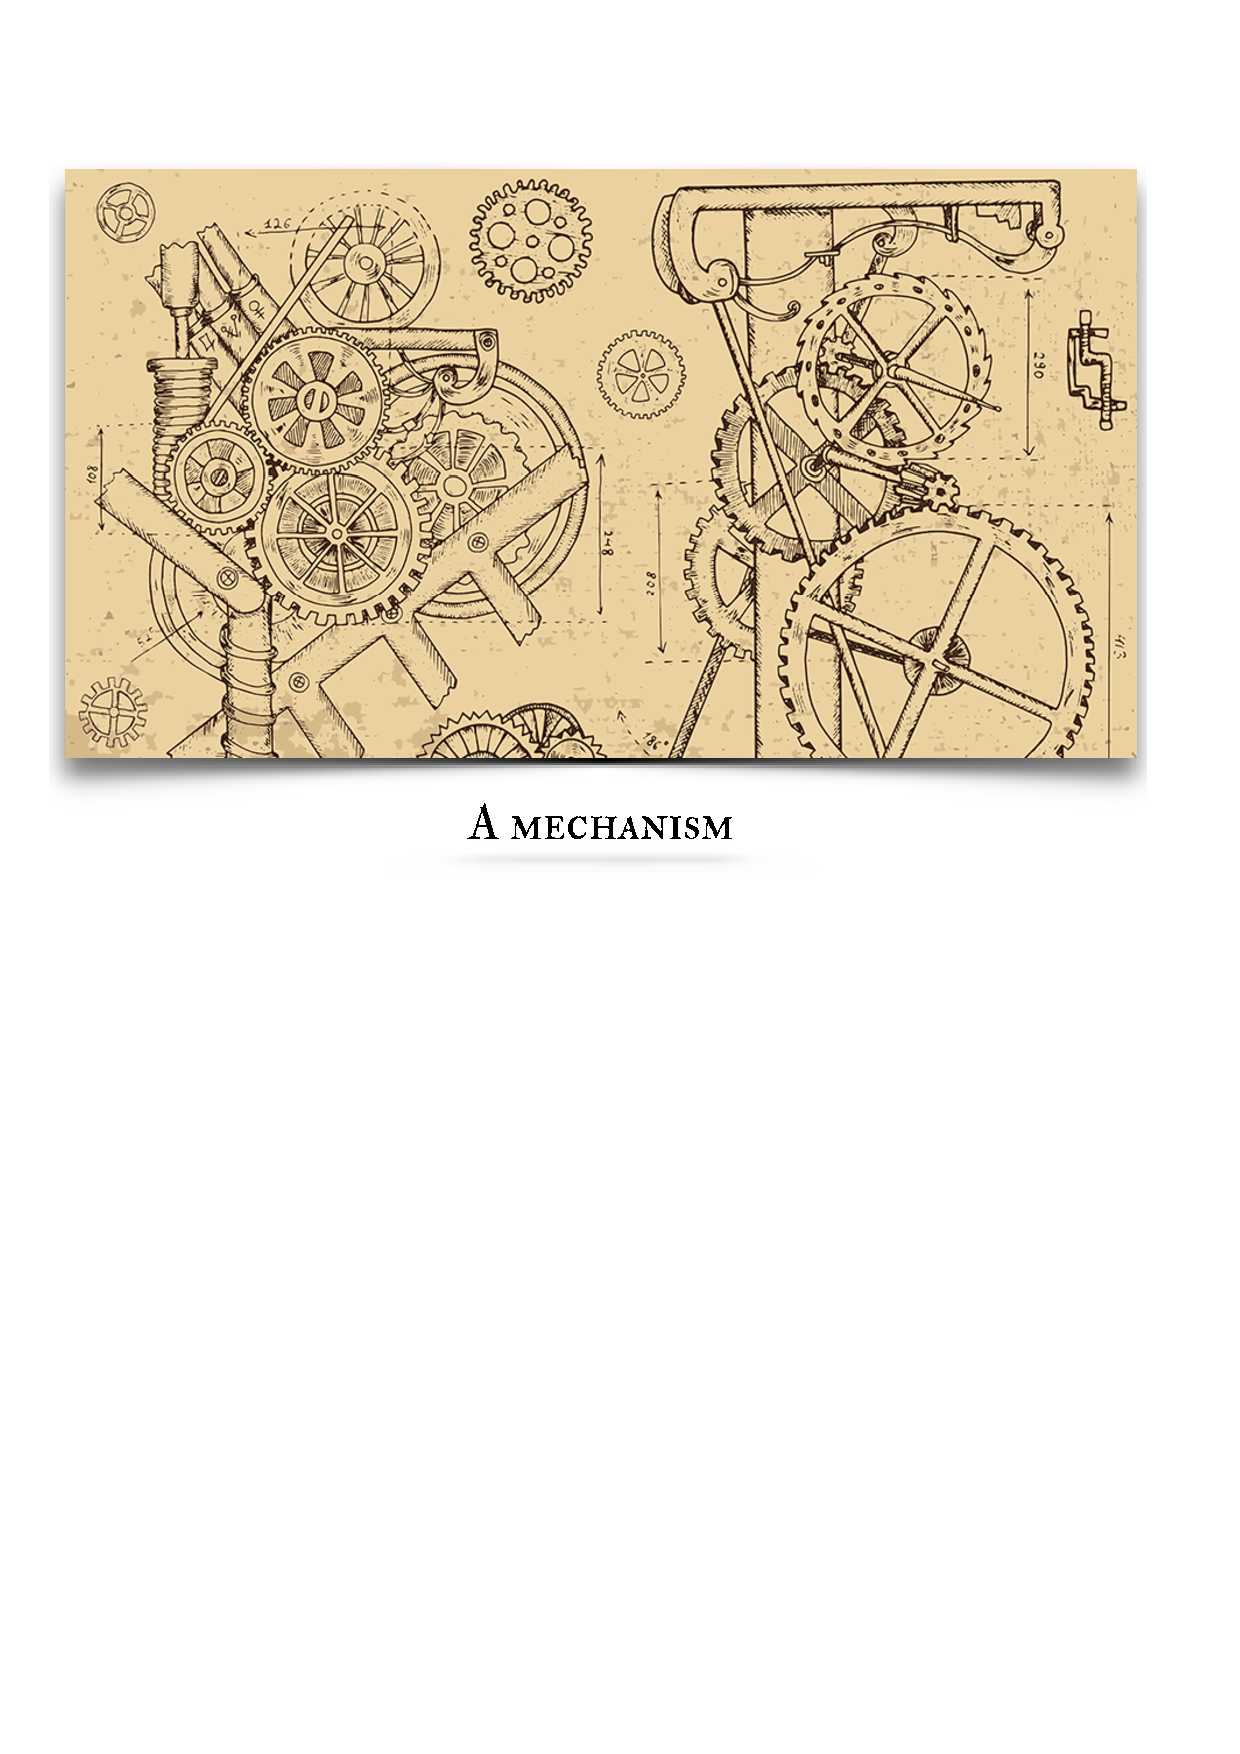
\includegraphics[width=\textwidth]{Figures/Mechanism.pdf}}
\vfill
